\documentclass{standalone}
\usepackage{tikz}
\usetikzlibrary{patterns, positioning}
\usepackage[sfdefault]{ClearSans} %% option 'sfdefault' activates Clear Sans as the default text font
\usepackage[T1]{fontenc}

\begin{document}
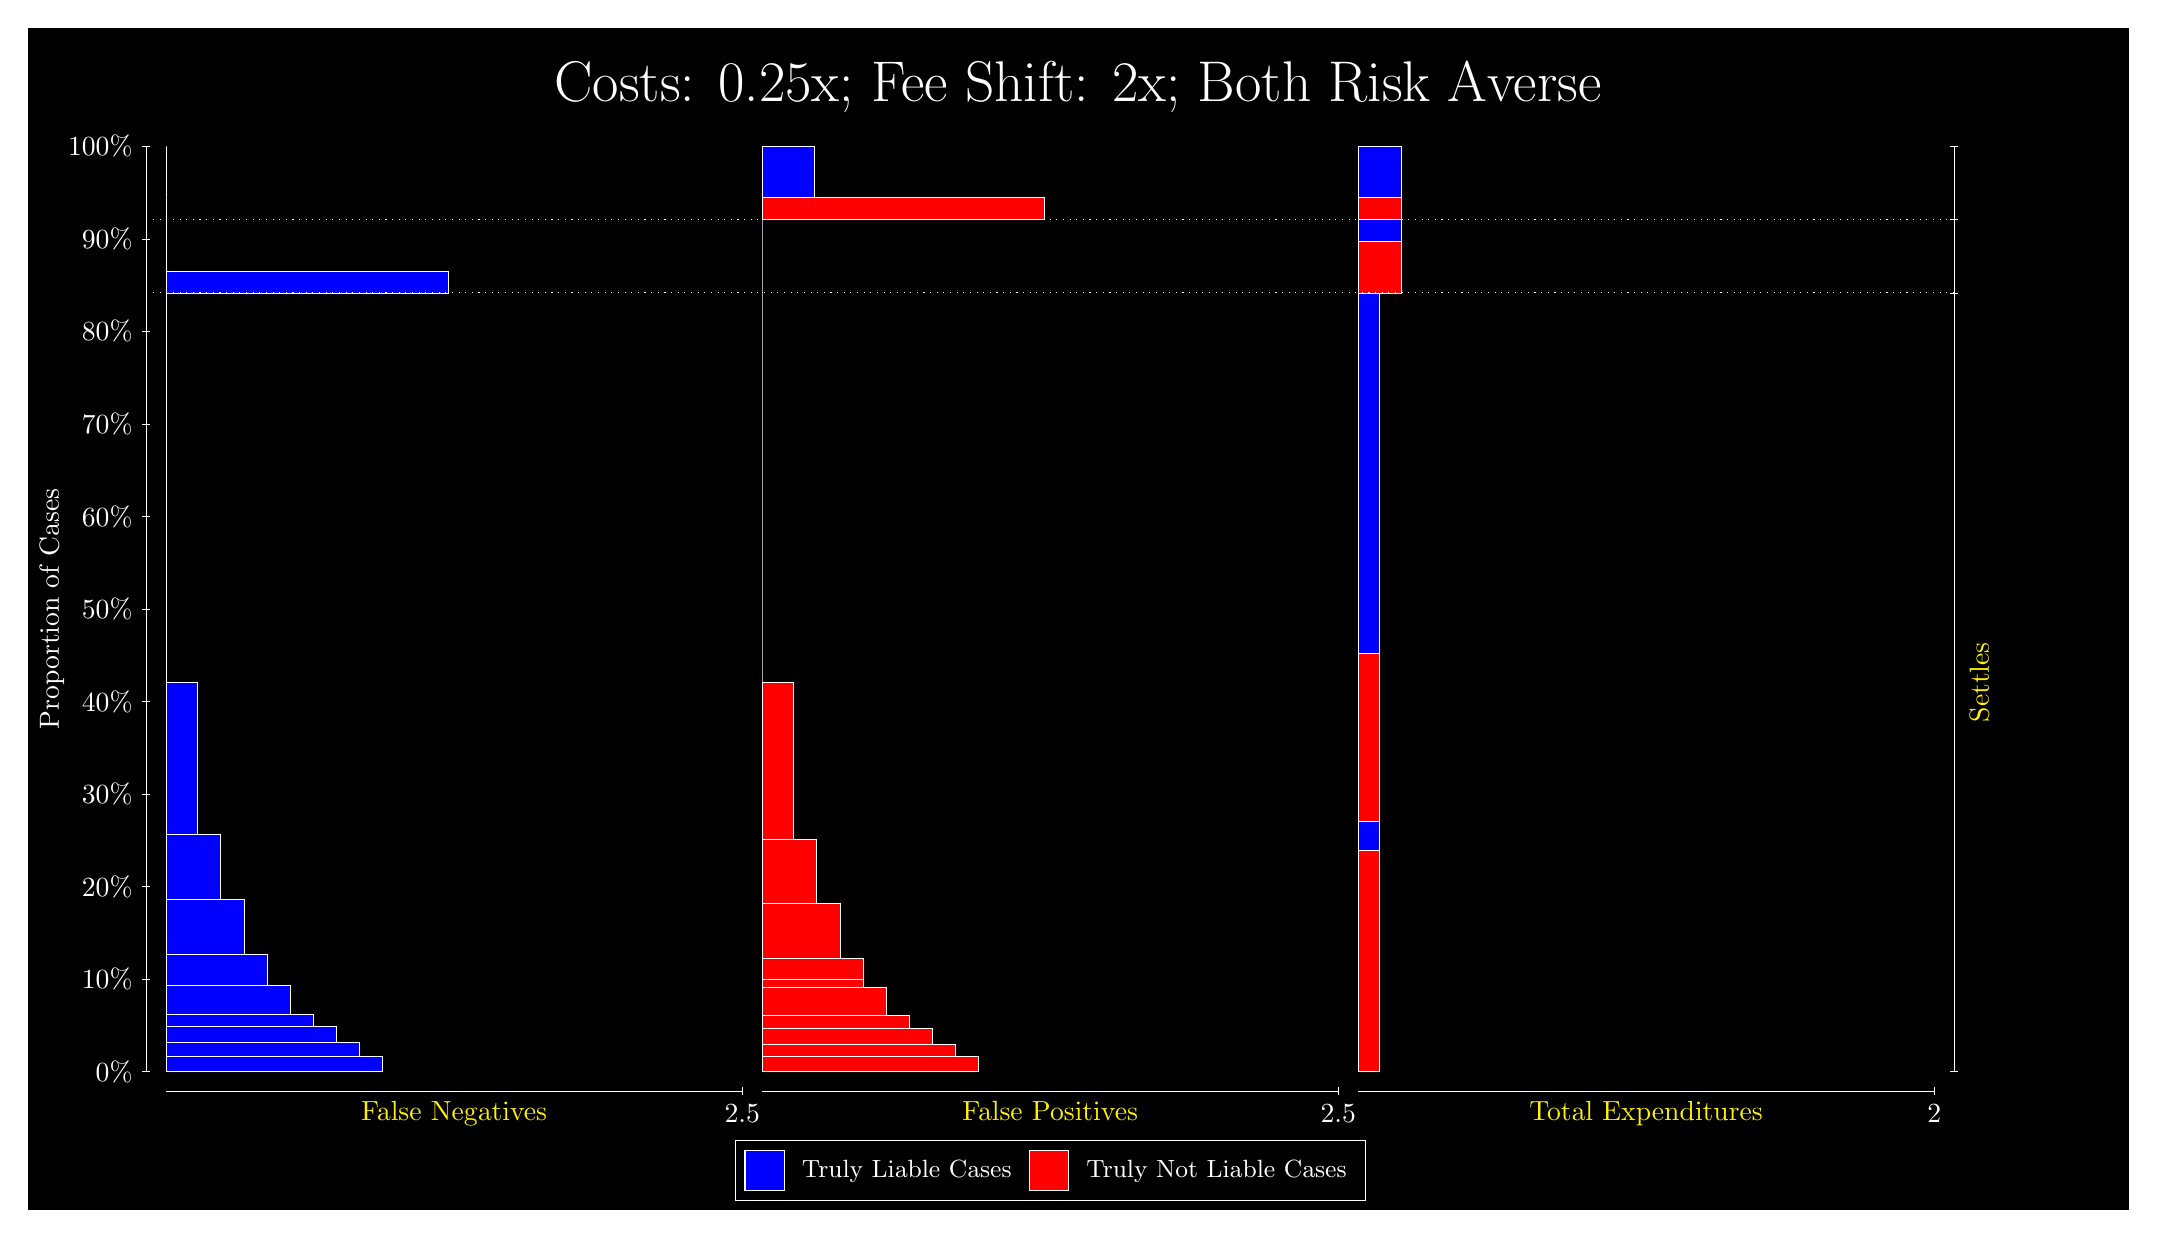
\begin{tikzpicture}
\draw[fill=black] (0,0) rectangle (26.667,15);
\draw[text=white] (0,13.5) rectangle (26.667,15) node[midway] {\huge Costs: 0.25x; Fee Shift: 2x; Both Risk Averse};
\draw[white, very thin] (1.5,1.75) -- (1.5,13.5);
\node[rotate=90, text=white, anchor=center] at (0.3, 7.625) {Proportion of Cases};
\draw[white, very thin] (1.45,1.75) -- (1.55,1.75);
\node[text=white, anchor=east] at (1.45, 1.75) {0\%};
\draw[white, very thin] (1.45,2.925) -- (1.55,2.925);
\node[text=white, anchor=east] at (1.45, 2.925) {10\%};
\draw[white, very thin] (1.45,4.1) -- (1.55,4.1);
\node[text=white, anchor=east] at (1.45, 4.1) {20\%};
\draw[white, very thin] (1.45,5.275) -- (1.55,5.275);
\node[text=white, anchor=east] at (1.45, 5.275) {30\%};
\draw[white, very thin] (1.45,6.45) -- (1.55,6.45);
\node[text=white, anchor=east] at (1.45, 6.45) {40\%};
\draw[white, very thin] (1.45,7.625) -- (1.55,7.625);
\node[text=white, anchor=east] at (1.45, 7.625) {50\%};
\draw[white, very thin] (1.45,8.8) -- (1.55,8.8);
\node[text=white, anchor=east] at (1.45, 8.8) {60\%};
\draw[white, very thin] (1.45,9.975) -- (1.55,9.975);
\node[text=white, anchor=east] at (1.45, 9.975) {70\%};
\draw[white, very thin] (1.45,11.15) -- (1.55,11.15);
\node[text=white, anchor=east] at (1.45, 11.15) {80\%};
\draw[white, very thin] (1.45,12.325) -- (1.55,12.325);
\node[text=white, anchor=east] at (1.45, 12.325) {90\%};
\draw[white, very thin] (1.45,13.5) -- (1.55,13.5);
\node[text=white, anchor=east] at (1.45, 13.5) {100\%};

\draw[white, very thin] (24.457,1.75) -- (24.457,13.5);
\draw[white, very thin] (24.407,1.75) -- (24.507,1.75);
\node[anchor=west] at (24.407, 1.75) {};
\draw[white, very thin] (24.407,11.64) -- (24.507,11.64);
\node[anchor=west] at (24.407, 11.64) {};
\draw[white, very thin] (24.407,12.568) -- (24.507,12.568);
\node[anchor=west] at (24.407, 12.568) {};
\draw[white, very thin] (24.407,13.5) -- (24.507,13.5);
\node[anchor=west] at (24.407, 13.5) {};

\draw[white, very thin, fill=blue] (1.75,1.75) rectangle (4.4946,1.949);
\draw[white, very thin, fill=blue] (1.75,1.949) rectangle (4.2018,2.1153);
\draw[white, very thin, fill=blue] (1.75,2.1153) rectangle (3.9091,2.3218);
\draw[white, very thin, fill=blue] (1.75,2.3218) rectangle (3.6163,2.4819);
\draw[white, very thin, fill=blue] (1.75,2.4819) rectangle (3.3236,2.8451);
\draw[white, very thin, fill=blue] (1.75,2.8451) rectangle (3.0308,3.2372);
\draw[white, very thin, fill=blue] (1.75,3.2372) rectangle (2.738,3.9327);
\draw[white, very thin, fill=blue] (1.75,3.9327) rectangle (2.4453,4.7651);
\draw[white, very thin, fill=blue] (1.75,4.7651) rectangle (2.1525,6.6929);
\draw[white, very thin, fill=red] (1.75,6.6929) rectangle (1.75,11.64);
\draw[white, very thin, fill=blue] (1.75,11.64) rectangle (5.3362,11.919);
\draw[white, very thin, fill=red] (1.75,11.919) rectangle (1.75,12.568);
\draw[white, very thin, fill=red] (1.75,12.568) rectangle (1.75,12.847);
\draw[white, very thin, fill=blue] (1.75,12.847) rectangle (1.75,13.5);
\draw[white, very thin, fill=red] (9.3189,1.75) rectangle (12.063,1.9374);
\draw[white, very thin, fill=red] (9.3189,1.9374) rectangle (11.771,2.0988);
\draw[white, very thin, fill=red] (9.3189,2.0988) rectangle (11.478,2.2939);
\draw[white, very thin, fill=red] (9.3189,2.2939) rectangle (11.185,2.4609);
\draw[white, very thin, fill=red] (9.3189,2.4609) rectangle (10.892,2.8241);
\draw[white, very thin, fill=red] (9.3189,2.8241) rectangle (10.6,2.9163);
\draw[white, very thin, fill=red] (9.3189,2.9163) rectangle (10.6,3.1884);
\draw[white, very thin, fill=red] (9.3189,3.1884) rectangle (10.307,3.8837);
\draw[white, very thin, fill=red] (9.3189,3.8837) rectangle (10.014,4.6956);
\draw[white, very thin, fill=red] (9.3189,4.6956) rectangle (9.7214,6.6969);
\draw[white, very thin, fill=blue] (9.3189,6.6969) rectangle (9.3189,11.64);
\draw[white, very thin, fill=red] (9.3189,11.64) rectangle (9.3189,12.289);
\draw[white, very thin, fill=blue] (9.3189,12.289) rectangle (9.3189,12.568);
\draw[white, very thin, fill=red] (9.3189,12.568) rectangle (12.905,12.847);
\draw[white, very thin, fill=blue] (9.3189,12.847) rectangle (9.9776,13.5);
\draw[white, very thin, fill=red] (16.888,1.75) rectangle (17.162,4.5632);
\draw[white, very thin, fill=blue] (16.888,4.5632) rectangle (17.162,4.9285);
\draw[white, very thin, fill=red] (16.888,4.9285) rectangle (17.162,7.0622);
\draw[white, very thin, fill=blue] (16.888,7.0622) rectangle (17.162,11.64);
\draw[white, very thin, fill=red] (16.888,11.64) rectangle (17.437,12.289);
\draw[white, very thin, fill=blue] (16.888,12.289) rectangle (17.437,12.568);
\draw[white, very thin, fill=red] (16.888,12.568) rectangle (17.437,12.847);
\draw[white, very thin, fill=blue] (16.888,12.847) rectangle (17.437,13.5);
\draw[white, dotted] (1.5,11.64) -- (24.457,11.64);
\draw[white, dotted] (1.5,12.568) -- (24.457,12.568);
\draw[white, very thin] (1.75,1.5) -- (9.0689,1.5);
\node[text=yellow, anchor=north] at (5.4094, 1.5) {False Negatives};
\draw[white, very thin] (9.0689,1.45) -- (9.0689,1.55);
\node[text=white, anchor=north] at (9.0689, 1.45) {2.5};

\draw[white, very thin] (9.3189,1.5) -- (16.638,1.5);
\node[text=yellow, anchor=north] at (12.978, 1.5) {False Positives};
\draw[white, very thin] (16.638,1.45) -- (16.638,1.55);
\node[text=white, anchor=north] at (16.638, 1.45) {2.5};

\draw[white, very thin] (16.888,1.5) -- (24.207,1.5);
\node[text=yellow, anchor=north] at (20.547, 1.5) {Total Expenditures};
\draw[white, very thin] (24.207,1.45) -- (24.207,1.55);
\node[text=white, anchor=north] at (24.207, 1.45) {2};

\node[text=yellow, centered, rotate=90] at (24.777, 6.6949) {Settles};



\draw (12.978300999999998,1.5) node[draw=none] (baseCoordinate) {};
\begin{scope}[align=center]
        \matrix[scale=0.5, draw=white, below=0.5cm of baseCoordinate, nodes={draw}, column sep=0.1cm]{
            \node[rectangle, draw, minimum width=0.5cm, minimum height=0.5cm, fill=blue] {}; &
            \node[draw=none, font=\small, text=white] (B) {Truly Liable Cases}; &
            \node[rectangle, draw, minimum width=0.5cm, minimum height=0.5cm, fill=red] {}; &
            \node[draw=none, font=\small, text=white] (B) {Truly Not Liable Cases}; \\
            };
\end{scope}

\end{tikzpicture}
\end{document}